% Selected supporting analyses; artwork and source checks: appendix-data/build.py.
\clearpage
\section*{Recovery relative to the stored ensemble}
\begin{figure}[htbp]
\centering
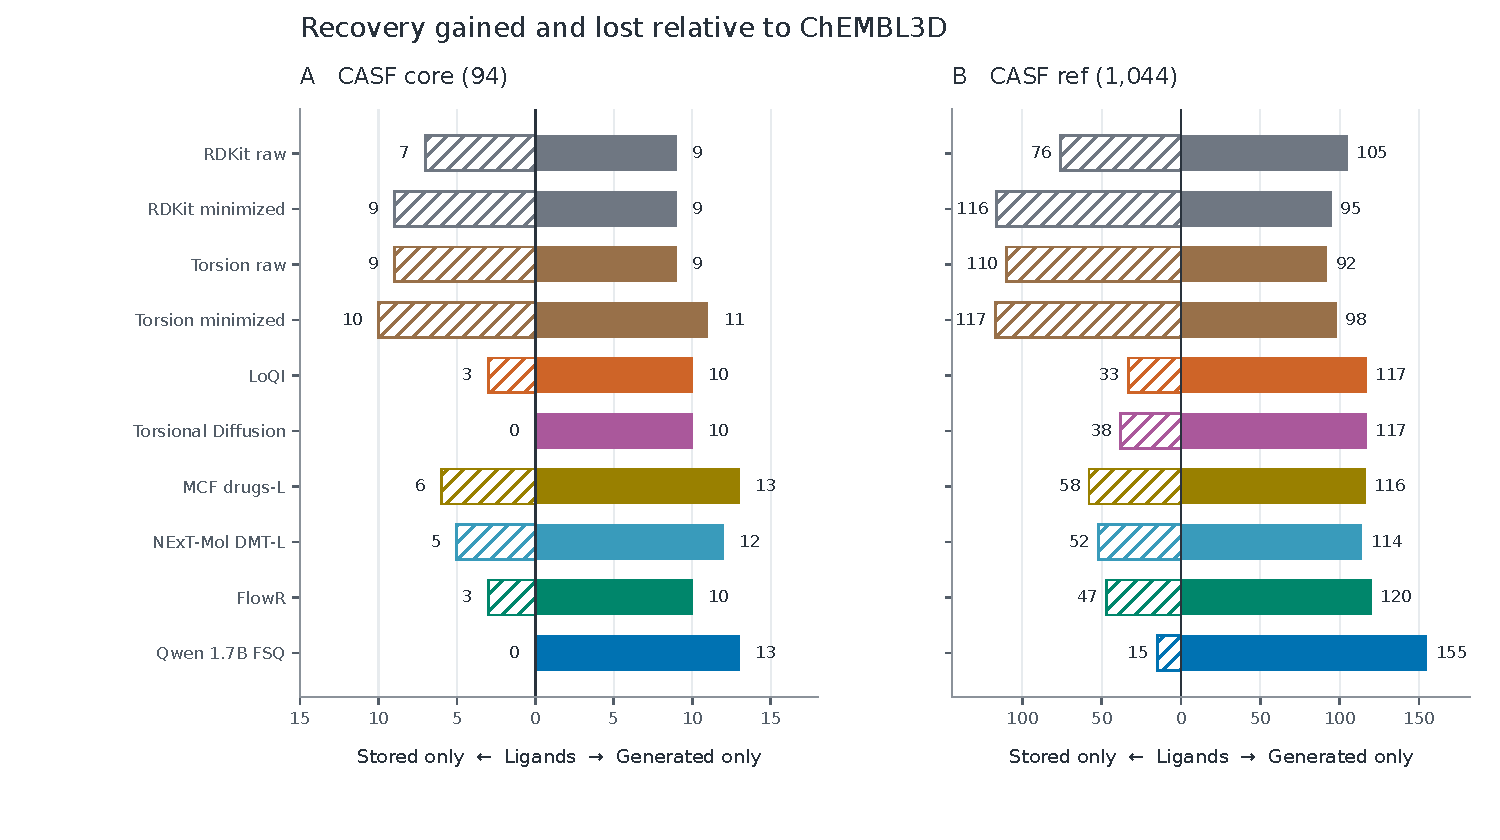
\includegraphics[width=\linewidth]{figures/supporting/recovery-gains-losses.pdf}
\caption{Recovery gained and lost relative to ChEMBL3D-PB on CASF core (A) and ref (B). Solid bars count ligands recovered only by the generated ensemble; hatched bars count ligands recovered only by the stored ensemble. Recovery requires a PoseBusters-passing conformer within 0.75~\AA{}. Generated ensembles use the 1,000-candidate target; the stored ensemble is unchanged. Shared hits and shared misses are omitted. Panel axes have different ranges.}
\label{fig:supporting-gains-losses}
\end{figure}

\clearpage
\section*{Joint composition of the CASF panels}
\begin{figure}[htbp]
\centering
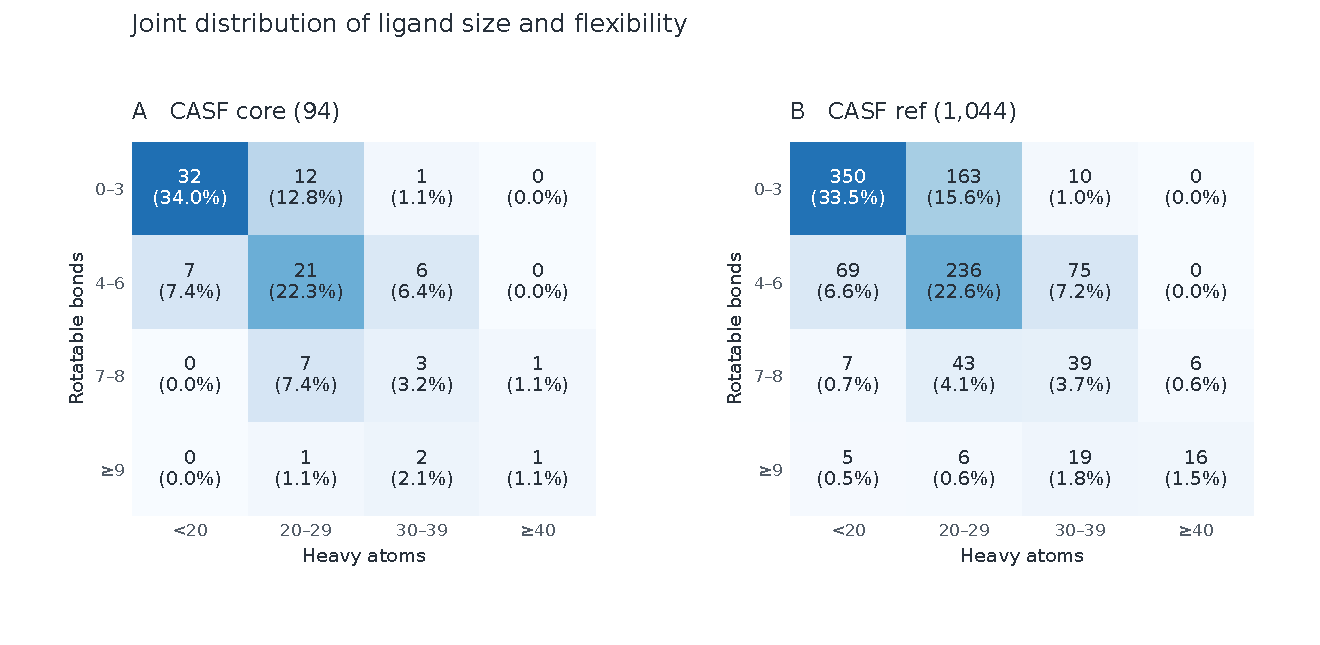
\includegraphics[width=\linewidth]{figures/supporting/cohort-composition.pdf}
\caption{Joint distribution of heavy-atom and rotatable-bond counts on CASF core (A) and ref (B). Cells give the number of ligands and percentage of the corresponding panel. Both panels use the same color scale for percentages. These are the reference-derived groups used in the main size and flexibility analysis. Empty and sparse combinations show the limits of evaluating size and flexibility independently.}
\label{fig:supporting-composition}
\end{figure}

\clearpage
\begin{landscape}
\begin{figure}[p]
\centering
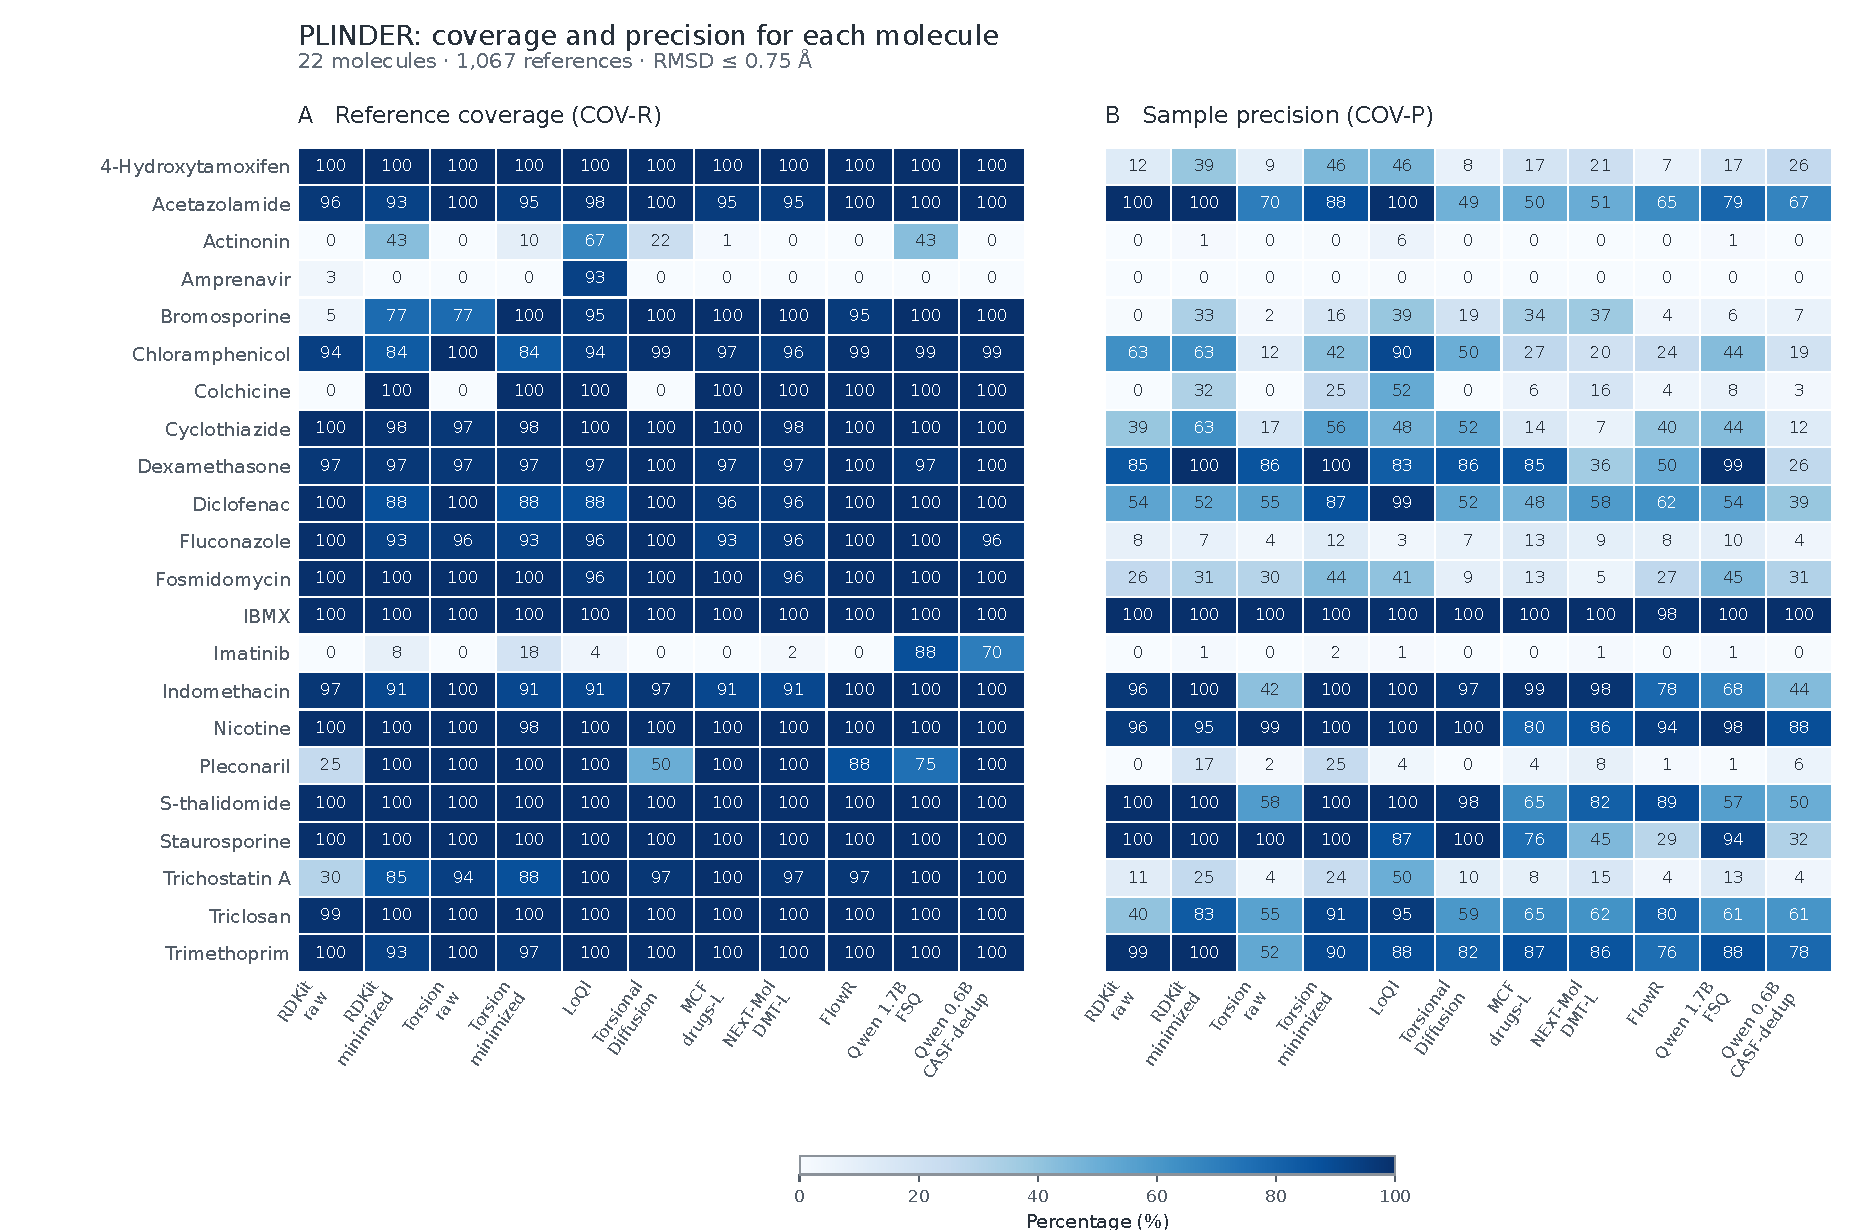
\includegraphics[width=0.98\linewidth,height=0.86\textwidth,keepaspectratio]{figures/supporting/plinder-coverage-precision.pdf}
\caption{Per-molecule PLINDER reference coverage (A) and sample precision (B) for the eleven methods in main Table 4. Both panels use RMSD $\leq0.75$~\AA{} and the full supplied conformer pools. Molecules have the same alphabetical ordering, and both panels share a 0--100\% scale. Values are rounded to whole percentages; displayed zeros and hundreds can include values just above zero or below 100. The torsion rows use the independent ETKDG starts.}
\label{fig:supporting-plinder-coverage}
\end{figure}
\end{landscape}

\clearpage
\begin{landscape}
\begin{figure}[p]
\centering
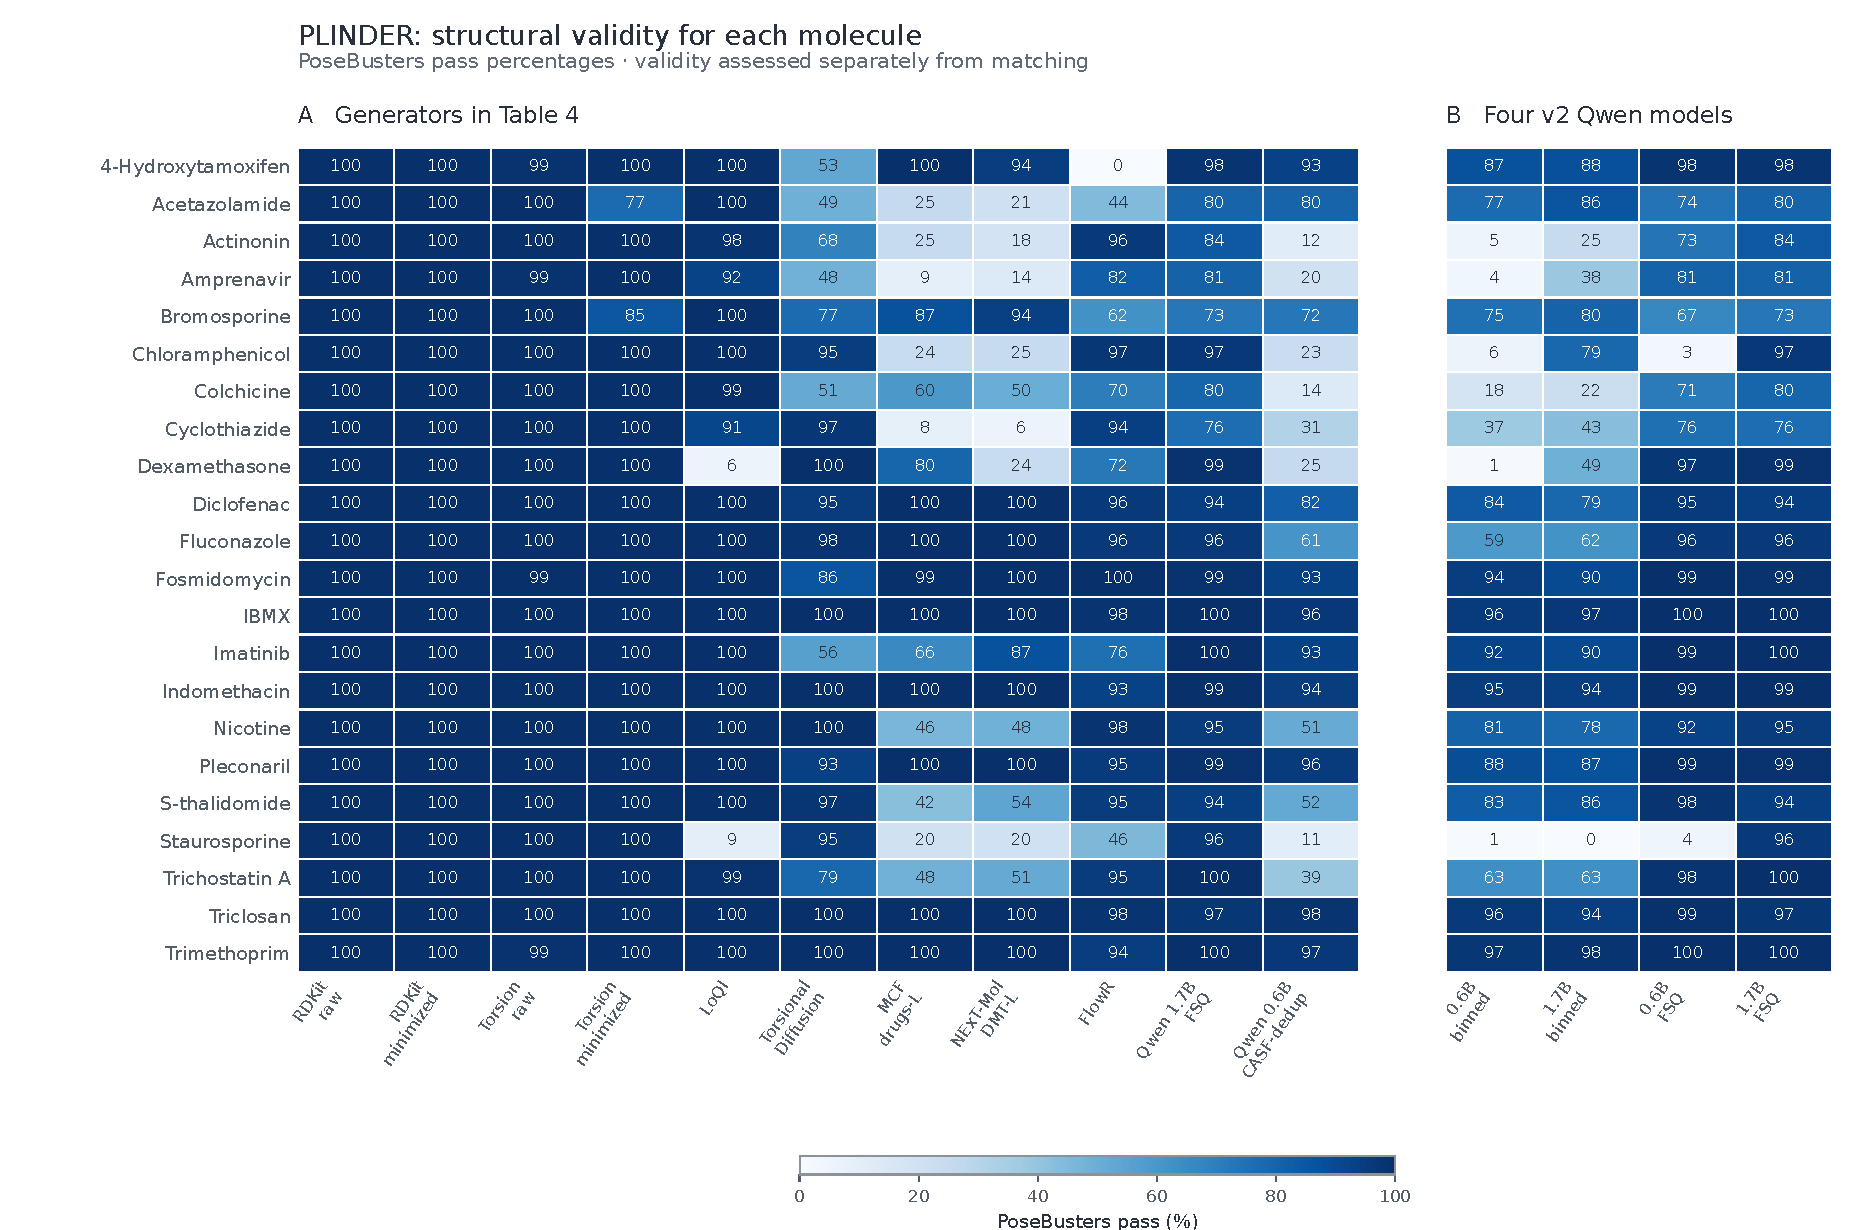
\includegraphics[width=0.98\linewidth,height=0.86\textwidth,keepaspectratio]{figures/supporting/plinder-validity.pdf}
\caption{Per-molecule PoseBusters pass percentages for the PLINDER generators in main Table 4 (A) and the four Qwen size/representation configurations in main Figure 8 (B). Validity is assessed separately from coverage and matching. Values are rounded to whole percentages on a common scale. The 0.6B CASF-dedup model in A is distinct from the binned 0.6B model in B; the primary 1.7B FSQ model appears in both panels. The same 22 molecular identities are used throughout.}
\label{fig:supporting-plinder-validity}
\end{figure}
\end{landscape}
